\iffalse
    \title{Assignment}
    \author{EE24BTECH11028}
    \section{EE}
    \chapter{2012}
  \fi

    \item Asuuming both the voltage sources are in phase,the value of $R$ for which maximum power is transferred from circult $A$ to circult $B$ is\\
%\begin{circuitikz}
    % Circuit A
 %   \draw (0,0) to[sV, v=$10\,V$] (0,-2);
  %  \draw ( 0,0) -- (1,0) to[R, l=$2\,\Omega$] (2,0) -- (3,0) to[R, l=$R$] (4,0)--(5,0) to[C, l=$-j1\,\Omega$] (5,-2)--(0,-2);

    % Circuit B
  %  \draw (2,0) -- (4,0) to[R, l=$R$] (4,-2) -- (2,-2);
   % \draw  (5,0) -- (8,0) to[sV, v=$3\,V$] (8,-2)--(5,-2);
%\end{circuitikz}\\
\begin{figure}[h!]
        \centering
        
\includegraphics[width=0.7\linewidth]{figure/fig1/fig1.pdf}
		\caption{}
        \label{stemplot}
\end{figure}
    \begin{enumerate}
        \item$0.8\ohm$\\
        \item$1.4\ohm$\\
        \item$2\ohm$\\
        \item$2.8\ohm$
     \end{enumerate}
     \item The state variable description of an $LTI$ system id given by \\
                           $\myvec{\dot{X_{1}}\\
                                \dot{X_{2}}\\
                                \dot{X_{3}}}=\myvec{
                                                     0 && a_{1} && 0\\
                                                     0 && 0 && a_{2}\\
                                                     a_{3} && 0 && 0 
                                }\myvec{
                                X_{1}\\
                                X_{2}\\
                                X_{3}
                                }+ \myvec{
                                0\\
                                0\\
                                1
                                }u$\\

                    $Y=\myvec{1 && 0 && 0}\myvec{X_{1}\\X_{2}\\X_{3}}$\\
        where Y is the output and u is the input.The system is controllable for 
        \begin{enumerate}
            \item$a_{1}\neq0$, $a_{2}=0$, $a_{3}\neq0$\\
            \item$a_{1}=0$, $a_{2}\neq0$, $a_{3}\neq0$\\
            \item$a_{1}=0$, $a_{2}\neq0$, $a_{3}=0$\\
            \item$a_{1}\neq0$, $a_{2}\neq0$, $a_{3}=0$ 
        \end{enumerate}
      \item The fourier transform of a signal $h\brak{t}$ is $H\brak{j\omega}=\frac{\brak{2\cos{\omega}}\brak{\sin {2\omega}}}{\omega}.$The value of $h\brak{0}$ is 
       \begin{enumerate}
           \item$\frac{1}{4}$
           \item$\frac{1}{2}$
           \item$1$\\
          \item$2$
       \end{enumerate}
       \item The feedback system shown below oscillates at 2 $\frac{rad}{s}$ when\\
    

\begin{figure}[h!]
        \centering
        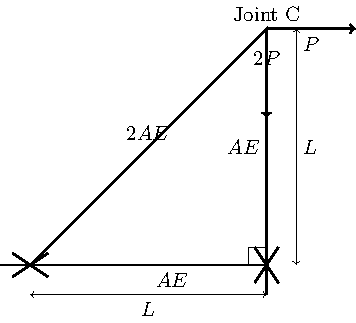
\includegraphics[width=0.7\linewidth]{figure/fig2/fig2.pdf}
		\caption{}
        \label{stemplot}
\end{figure}
     \begin{enumerate}
         \item$K=2$ and $a=0.75$\\
         \item$K=3$ and $a=0.75$\\
         \item$K=4$ and $a=0.5$\\
         \item$K=2$ and $a=0.5$
          \end{enumerate}
    \item The input $X\brak{t}$ and output $Y\brak{t}$ of the system are related as $y\brak{t}=\int_\infty^tX\brak{\tau}\cos\brak{3\tau}\mathrm{d}\tau$.The system is\\
    \begin{enumerate}
        \item time-invariant and stable\\
        \item stable and not time-invariant\\
         \item time-invariant and notstable\\
        \item not time-invariant and not stable
    \end{enumerate}
    \item An analog voltage uses external multiplier settings.With a multiplier setting of 2$0 K\ohm$,it reads $440 V$ and with a multiplier setting of $80 K\ohm$,its reads $352 V$.For a multiplier setting of $40 K\ohm$, the voltmeter reads\\
    \begin{enumerate}
        \item$371 V$\\
        \item$383 V$\\
        \item$394 V$\\
        \item$406 V$
    \end{enumerate}
    \item The locked rotor current in a $3$-phase, star connected $15 KW$, $4$-pole, $230 V$, $50Hz$ induction motor at rated conditions is $50 A$.Neglecting losses and magnetizing current, the approximate looked rotor line  current draw when the motor is connected to a $236 V$, $57 Hz$ supply is\\
    \begin{enumerate}
        \item$58.8 a$\\
        \item$45.0 A$\\
        \item$42.7 A$\\
        \item$55.6 A$
    \end{enumerate}
    \item A singal phase $10 KV A$, $50 Hz$ transformer with $1 KV$ primary winding draws $0.5 A$ and $55 W$, at rated voltage and frequency, on no load . A second transformer has a core with its linear dimensions $\sqrt{2}$ times the corresponding dimsensions of the first transformer.The core material and lamination thickness are the same in both transformers.The primary winding of both the transformers have the same number of turns. If a rated voltage of $2 KV$ at $50 Hz$ is applied to the primary of the second transformer, then the no load current and power, respectively, are\\
    \begin{enumerate}
        \item$0.7 A$, $77.8 W$\\
        \item$0.7 A$, $155.6 W$\\
        \item$1 A$, $100 W$\\
        \item$1 A$, $200 w$
    \end{enumerate}
    Common Data Question\\
    Common Data for Question $48$ and $49$\\
    In the 3-phase inverter circult shown, the load is balanced and the gating scheme is $180\degree$-conduction mode.All the switching devices are ideal.
    \begin{figure}[h!]
        \centering
        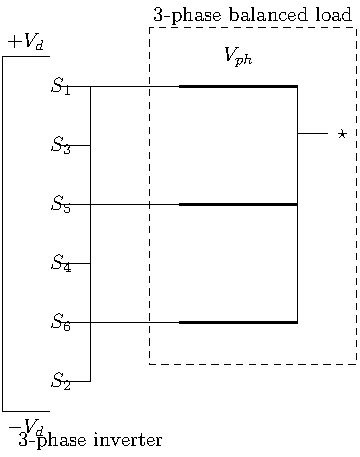
\includegraphics[width=0.7\linewidth]{figure/fig3/fig3.pdf}
		\caption{}
        \label{stemplot}
\end{figure}
\item The rns value of load phase voltageis 
\begin{enumerate}
    \item$106.1 V$\\
    \item$141.4 V$\\
    \item$212.2 V$\\
    \item$282.8 V$
\end{enumerate}
\item If the dc bus voltage $V_{d}=300 V$, the power consumed by $3$-phase load is
\begin{enumerate}
    \item$1.5 kW$\\
    \item$2.0 kW$\\
    \item$2.5 kW$\\
    \item$3.0 kW$
\end{enumerate}
       Common Data for Question $50$ and $51$\\
         With $10 V$ dc connected at port $A$ in linear nonrecirocal two-port network shown below, the following were observed\\
         $\brak{i}1\ohm$ connected at port B draws a current of $3 A$\\
           $\brak{ii}2.5\ohm$ connected at port B draws a current of $2 A$\\
           
\begin{figure}[h!]
        \centering
        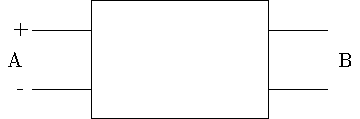
\includegraphics[width=0.7\linewidth]{figure/fig4/fig4.pdf}
		\caption{}
        \label{stemplot}
\end{figure}
\item For the same network, with $6 V$ dc connected at port $A$, $1\ohm$ connected at port $B$ draws $\frac{7}{3} A$.If $8 V$ dc connected to port $A$, the open circult voltage at port $B$ is 
\begin{enumerate}
    \item$6 V$\\
    \item$7 V$\\
    \item$8 V$\\
    \item$9 V$
    \end{enumerate}
    \item With $10 V$ dc connected at port $A$, the current drawn by $7\ohm$ connected at port $B$ is
    \begin{enumerate}
        \item$\frac{3}{7}A$\\
         \item$\frac{5}{7}A$\\
        \item$1 A$\\
        \item$\frac{9}{7}A$
    \end{enumerate}
    \item In the circuit shown,the three voltage reading are $V_{1} = 220 V$ , $V_{2} = 122 V$, $V_{3} = 136 V$.The power factor of the load is\\
 \begin{figure}[h!]
        \centering
        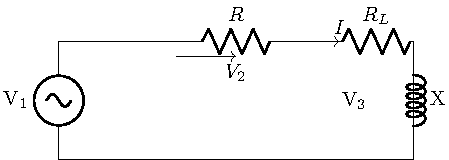
\includegraphics[width=0.7\linewidth]{figure/fig5/fig5.pdf}
		\caption{}
        \label{stemplot}
\end{figure}
\begin{enumerate}
    \item$0.45$\\
    \item$0.50$\\
    \item$0.55$\\
    \item$0.60$
\end{enumerate}


   
